\documentclass[pdftex,12pt,a4paper]{report} 

% Document settings

\usepackage{fullpage}
\usepackage{cite}
\usepackage{datetime} 
\usepackage{geometry}
\usepackage[pdftex]{graphicx}
\usepackage{verbatim}
\usepackage{todonotes}

\geometry{verbose,lmargin=3cm,rmargin=3cm}

\newcommand{\HRule}{\rule{\linewidth}{0.5mm}}

\begin{document}

\section{GUI}

\paragraph{Choice of Language}
For the GUI the HaXe programming language (together with the NME library) was chosen so as to be able to build a cross-platform GUI capable of use on Windows/Mac/Linux desktops as well as Android and OSX mobile devices without worrying about each individual plaform and it's capabilities.

\paragraph{Capabilities}
The GUI is fully DAIDE compliant and able to observe a Diplomacy game played on any DAIDE compliant server.

Unit locations, supply centre ownerships and moves are all displayed to the user on a scrolling/zoomable map with the whole GUI resizable to any reasonable dimension.

Game view is controlled by playback buttons with the ability to step through turns individually or view the game at a controllable pace. These are placed in the title bar together with the connection interface. \\[0.5cm]

\includegraphics[scale=0.5]{./screenshots/Titlebar.png} \\[0.5cm]
This titlebar also displays the current turn/phase of the game being viewed.

\paragraph{CLI}
The GUI includes a command line interface which can be overlayed on the map providing resources for debugging moves and inputting moves manually as a human-player (Ontop of which like the GUI itself, a human-player GUI can be implemented).

\paragraph{Flexibility}
The GUI is capable of playing/observing a game on any Map, and is preloaded with the required resources for playing the standard DAIDE map.

Each map to be used in the GUI requires:
\begin{itemize}
\item{An .svg vector graphic file which provides graphic paths for clickable regions of the map (Selection of regions is implemented in the GUI but disabled once it was decided there was insufficient time to implement a human player GUI). Together with a set of named graphics to encode the locations that units may occupy and supply centre locations.

SVG is a widely-deployed, royalty-free graphics format with an open specification based on .xml files and can be created by many graphics editors.

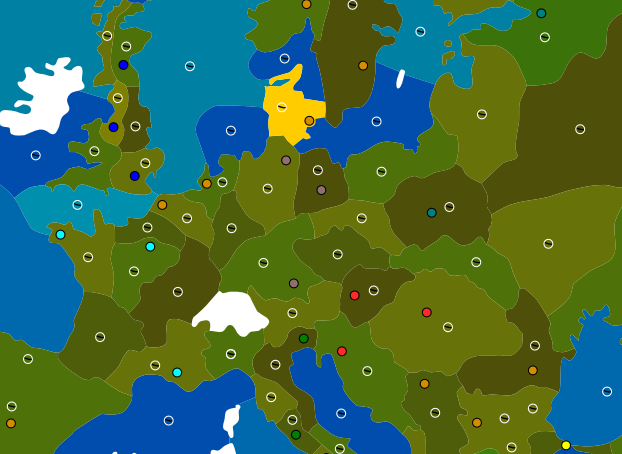
\includegraphics[scale=0.5]{./gui/SVG.png}
Note that colours and shape/size of location markers are arbitrary. Information to be mapped to the real DAIDE map is supplied in metadata.}
\item{A simple text file mapping province names used in the SVG file metadata, to DAIDE protocol IDs}
\item{A set of graphics to be used with trilinear filtering to provide crisp display of the map at any zoom level with little performance loss compared to runtime rendering of a detailed and complex vector graphic for instance.}

\end{itemize}

\paragraph{Technical Issues}
As with the Haskell AI, it was necessary to implement a full implementation of the DAIDE protocol including serialisation/deserialisation of DAIDE tokens, and parseing/unparsing of language constructs. As the GUI was first started with the CLI it was necessary also to build a lexer for DAIDE tokens from their textual representations and for debug purposes in communicating with the server.

For these tasks existing open-source HaXe libraries (hlex,hllr) were used (And extended to provide more type safety in the parser to help with a grammar as large as that of DAIDE).

Additionally, there is no existing .svg library for HaXe. A reader for the subset of the SVG format required for the GUI was thus written, including the transformation of graphic paths into a more suitable format for mouse selection.

The NME library itself was also forked onto github for the purposes of providing an extension to it's features used in the GUI.

\paragraph{Design}
The GUI was seperated into 3 packages seperating concerns of the DAIDE protocol, SVG and other map data, and the GUI itself.\\[0.5cm]
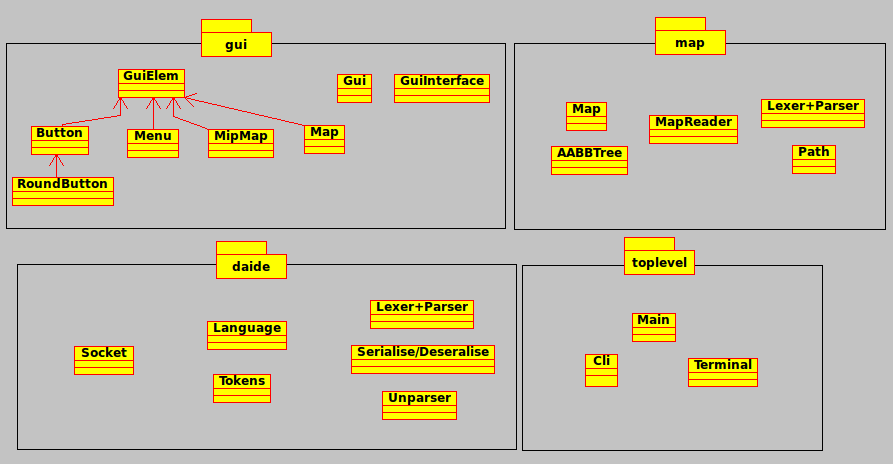
\includegraphics[scale=0.5]{./gui/UML.png}\\[0.5cm]
\begin{itemize}
\item{The gui package encloses all parts of the real GUI including it's interface to the DAIDE socket.}
\item{The daide package encloses everything to do with lexing/parsing/serialisation of the DAIDE messages together with a wrapper around an Asynchronous TCP socket handling the low-level DAIDE protocol dispatching messages to the GUI interface and receiving any messages to be sent to the server.}
\item{The map package encloses everything to do with reading .svg files and other related files for maps, together with a struct for enclosing all map information for rendering and though no unsued, a fast aabb tree for quickly selecting which polygons reprsenting regions are to be tested in mouse selection.}
\item{The toplevel package includes the very small Main class instantiating the GUI, CLI and Terminal and binding them together, the Terminal being a simple gui in its own right providing textual input for the CLI used by both the Terminal and the GUI interface.}\\[1cm]
\end{itemize}
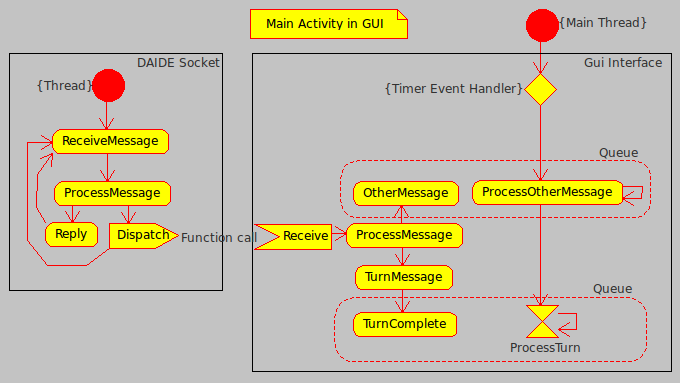
\includegraphics[scale=0.5]{./gui/Activity.png}\\[0.5cm]
The entire GUI operates on 2 threads.

The Main thread which deals with most of the work, specifically all GUI related work as demanded by the NME library which is not thread safe.

The DAIDE socket thread deals with receiving messages from the server and can reply to basic low-level DAIDE protocol, sending any complex messages to the GUI Interface to be processed and entered into one of two areas:
\begin{itemize}
\item{A queue for any non-turn related messages which are processed whenever possible by the Timer Event handler forming part of the GUI Interface}
\item{A queue for completed turn records, with any message forming part of an on-going turn being accumulated into a record before being pushed onto the queue. The handling of this queue in the GUI Interface Timer Event handler deals with being in a paused/playing state and any delays necessary to keep the speed set by the UI}
\end{itemize}


\end{document}
